\documentclass[tikz,border=2]{standalone}
%% \usepackage{amsfonts}
\usepackage{lmodern} % enhanced version of computer modern
\usepackage[T1]{fontenc} % for hyphenated characters
\usepackage{amssymb}
\usepackage{amsmath}
\usepackage{amsthm}
%
\usepackage{ctable}
\usetikzlibrary{decorations.pathreplacing,shadows,arrows,shapes,positioning,calc,backgrounds,fit}
\newcommand{\mA}{\mathcal{A}}
\newcommand{\mB}{\mathcal{B}}
\newcommand{\mC}{\mathcal{C}}
\newcommand{\mI}{\mathcal{I}}
\newcommand{\mN}{\mathcal{N}}
\newcommand{\mP}{\mathcal{P}}
\newcommand{\mR}{\mathcal{R}}
\newcommand{\mS}{\mathcal{S}}
\newcommand{\mY}{\mathcal{Y}}
% Define the layers to draw the diagram
%
\begin{document}
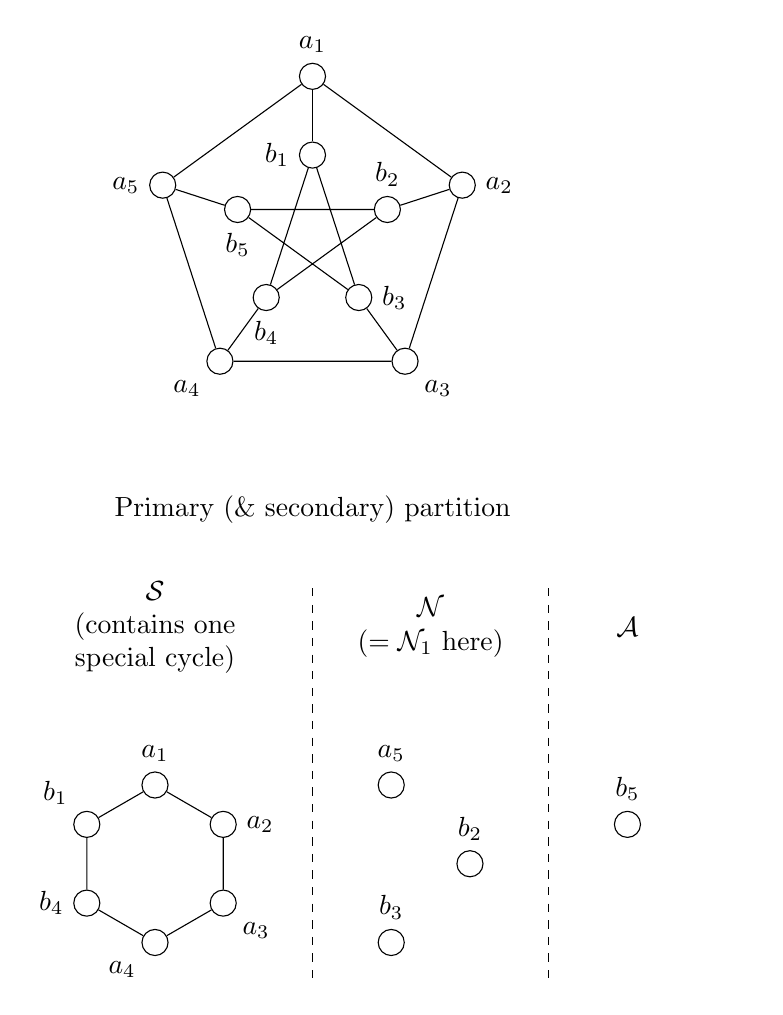
\begin{tikzpicture}
[node distance=1cm,
vert/.style={draw,circle,fill=white},
N/.style={circle,fill=black},
dedge/.style={black,>=latex', shorten >=.0pt, shorten <=.0pt},
edge/.style={}]
%% Graph
% outer circle
\def \n {5}
\def \rad {2cm}
\node[vert,label=above:$a_1$] (a1) at ({360/\n * 0+90}:\rad) {};
\node[vert,label=right:$a_2$] (a2) at ({360/\n * -1+90}:\rad) {};
\node[vert,label=below right:$a_3$] (a3) at ({360/\n * -2+90}:\rad) {};
\node[vert,label=below left:$a_4$] (a4) at ({360/\n * -3+90}:\rad) {};
\node[vert,label=left:$a_5$] (a5) at ({360/\n * -4+90}:\rad) {};
% inner circle
\def \n {5}
\def \rad {1cm}
\node[vert,label=left:$b_1$] (b1) at ({360/\n * 0+90}:\rad) {};
\node[vert,label=above:$b_2$] (b2) at ({360/\n * -1+90}:\rad) {};
\node[vert,label=right:$b_3$] (b3) at ({360/\n * -2+90}:\rad) {};
\node[vert,label=below:$b_4$] (b4) at ({360/\n * -3+90}:\rad) {};
\node[vert,label=below:$b_5$] (b5) at ({360/\n * -4+90}:\rad) {};
% edges
%\begin{pgfonlayer}{background}
\draw[edge] (a1) -- (a2) -- (a3) -- (a4) -- (a5) -- (a1);
\draw[edge] (b1) -- (b4) -- (b2) -- (b5) -- (b3) -- (b1);
\draw[edge] (a1) -- (b1);
\draw[edge] (a2) -- (b2);
\draw[edge] (a3) -- (b3);
\draw[edge] (a4) -- (b4);
\draw[edge] (a5) -- (b5);
%\end{pgfonlayer}
%%%%%%%%%%%%%%%%%%%%%%%%%%%%%
%% Decomposition
\begin{scope}[xshift=-2cm,yshift=-5cm]
\node at (2,1.5) {Primary (\& secondary) partition};
% partition S
\node at (0,0) {\parbox{3cm}{\centering $\mS$ \\ (contains one special cycle)}};
\begin{scope}[xshift=0cm,yshift=-3cm]
\def \n {6}
\def \rad {1cm}
\node[vert,label=above:$a_1$] (a1) at ({360/\n * 0+90}:\rad) {};
\node[vert,label=right:$a_2$] (a2) at ({360/\n * -1+90}:\rad) {};
\node[vert,label=below right:$a_3$] (a3) at ({360/\n * -2+90}:\rad) {};
\node[vert,label=below left:$a_4$] (a4) at ({360/\n * -3+90}:\rad) {};
\node[vert,label=left:$b_4$] (b2) at ({360/\n * -4+90}:\rad) {};
\node[vert,label=above left:$b_1$] (b1) at ({360/\n * -5+90}:\rad) {};
%
\draw[edge] (a1) -- (a2) -- (a3) -- (a4) -- (b2) -- (b1) -- (a1);
%
\end{scope} % S
%%
% partition N
\node at (3.5,0) {\parbox{3cm}{\centering $\mN$\\ ($=\mN_1$ here)}};
\begin{scope}[xshift=4cm,yshift=-3cm]
\node[vert,label=above:$a_5$] (a5) at (-1,1) {};
\node[vert,label=above:$b_2$] (b3) at (0,0) {};
\node[vert,label=above:$b_3$] (b5) at (-1,-1) {};
%
\end{scope} % N
%
% partition A
\node at (6,0) {\parbox{3cm}{\centering $\mA$}};
\begin{scope}[xshift=6cm,yshift=-3cm]
\node[vert,label=above:$b_5$] (b4) at (0,0.5) {};
%
\end{scope} % N
%
\draw[dashed] (2,.5) -- +(0,-5) {};
\draw[dashed] (5,.5) -- +(0,-5) {};
\end{scope} % decomposition
%%%%%%%%%%%%%%%%%%%%%%%%%%%%
\end{tikzpicture}
{}
\end{document}
